%TODO: MarginPARS zetten
%TODO: Figuur plaatsing Bas Broere vragen.
\chapter{Onderzoeksmethode}\label{ch:onderzoeksmethode} % Chapter title

Op basis van de requirements analyse beschreven in het vorige deel zijn er een aantal vragen ontstaan die verder onderzoek behoeven. Er is gekozen om het onderzoek op te delen in drie delen, waarbij iedere deel in een eigen hoofdstuk wordt beschreven. De Onderwerpen zijn gekozen omdat ze kennis verschaffen welke in het ontwerp van de nieuwe oplossing.

Als eerste dient er gekeken worden hoe er binnen EagleScience software ontwikkeld en uitgerold wordt. Deze kennis is nodig om te zien of er aanpassingen gedaan kunnen worden binnen de huidige methode en/of uitrolstraat. Daarnaast geeft het inzicht in de gebruikte platformen en daarbij de architectuur waarin er een applicatie moet worden ontwikkeld. Om verder inzicht te verkrijgen in de materie rondom SOUP en de gevaren van die het potentieel met zich meebrengt dient er onderzoek gedaan te worden naar dit onderwerp. Als laatste dient er een onderzoek gedaan te worden naar de mogelijkheden om een analyse te doen binnen de gebruikte architectuur van EagleScience. Hierin moet worden gekeken naar externe bibliotheken en/of tooling die aangemerkt zijn als veilig. Het laatste onderzoek in dit deel bevat alle resultaten samen. Dit hoofdstuk kan als ingang worden gebruikt voor het ontwerp en de implementatie welke beschreven is in het volgende deel.

In dit hoofdstuk zal er worden gekeken naar de onderzoeks methoden voor de drie onderzoeken. HEt zal ingaan op de scope, gebruikte bronnen en technieken om deze onderzoeken te doen.
%aantal vragen ontstaan die verder onderzoek benodigd behoeven. In dit deel worden de vragen geanalyseerd en beantwoord zodat er een duidelijkheid is in de materie en een goede basis wordt gelegd voor de daadwerkelijke implementatie beschreven in het volgende deel. Er is gekozen om het vooronderzoek in drie hoofdstukken op te delen omdat ieder deel onderzoek een eigen uitgesproken onderwerp heeft. Zeker het onderzoek naar de manier van werken binnen EagleScience staat in zeker los van de thee hoofdstukken over cybersecurity en later over methodes om bibliotheken te analyseren. Echter is de informatie die het resultaat is van het ene onderzoek input voor het onderzoek erna. Door eerst te kijken naar de manier waarop Eaglescience werkt kan die als een scope dienen voor de onderzoeken die er na uitgevoerd worden.
%
%Om verder inzicht te krijgen in de materie rondom de opdracht is er onderzoek nodig. Er worden drie onderzoek gedaan die ieder zijn eigen onderwerp hebben. Gezamelijk zorgen ze voor input voor het ontwerp en de daadwerkelijke implementatie. In dit hoofdstuk word ingegaan op de manier waarop de onderzoeken zijn uitgevoerd en welk doel zei hebben. Daarna volgt er voor ieder onderzoek een eigen hoofdstuk die het onderwerp behandeld en met resultaten komt. Als laatst is er een algehele conclussie die als input dient voor het ontwerp van de implementatie.


\section{Scope}\label{sec:Scope}
Software veiligheid is een breed gebied met veel relevante onderwerpen binnen het ontwikkelen van software. Echter gezien de gewenste oplossing alleen inzicht geeft in gevaren die met zich meebrengen
Het onderzoek zal zich beperken tot de benodigde informatie voor het implementeren van de nieuwe oplossing voor een geautomatiseerde SOUP analyse. Hierdoor zullen andere onderwerpen binnen het veilig ontwerpen van software niet worden onderzocht. Zo zullen ook niet alle bedrijfprocessen binnen EagleScience worden onderzocht en alleen gekeken worden naar de processen binenn het uitrollen van de software. EagleScience doet veel aan het veilig ontwerpen van zijn eigen ontwikkelde software waardoor de noodzaak op het moment van het geven van de opdracht niet hoog ligt.


\section{Onderzoek 1: Architectuur binnen EagleScience}\label{sec:onderzoeksmethode-architectuur-binnen-eaglescience}
Het \textbf{doel} van dit onderzoek is om kennis te vergaren over de manier van uitrollen van software binnen EagleScience. Daarnaast moet het onderzoek inzicht geven in de gebruikte dev-stack( programeertalen, tooling en frameworks). De uitkomst is relevant omdat het een basis is waar de nieuwe oplossing werkzaam in moet zijn. De \textbf{methodes} die gebruikt worden zijn de interne documenten over de verschillende platformen en werkwijzen die beschikbaar zijn gesteld door het bedrijf zelf. De kennis uit deze documenten kan worden aangevuld door informatie welke verstrekt is door de leveranciers. Daarnaast zullen er gesprekken plaats vinden met collega's. Deze input geeft het volgende onderzoeks model wat te zien is in figuur~\ref{fig:OnderzoeksModelEaglescience}
De \textbf{bronnen} die voornamelijk gebruikt worden zijn interne documenten waarin vermeld staat hoe een project verloopt en welke tooling er gebruikt wordt. Daarnaast zal er veel gebruik gemaakt worden van kennis van collega's en die ik zelf heb opgedaan dan al niet tijdens mijn opleiding.
\begin{figure}[htbp] %todo: Nog in kleur zetten van Eaglescience als deze goed is.
    \myfloatalign
    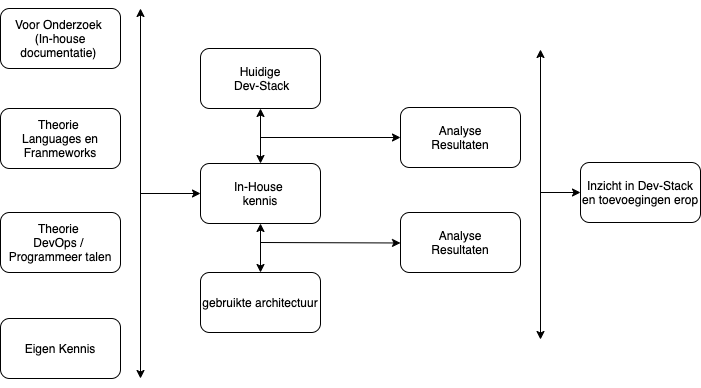
\includegraphics[width=10cm]{gfx/OnderzoeksmodelES}
    \caption{Onderzoeksmodel Eaglescience}
    \label{fig:OnderzoeksModelEaglescience}
\end{figure}


\newpage % quickfix om volgordelijkheid te veranderen voor figuren...


\section{Onderzoek 2: Literatuur studie veiligere software door SOUP analyse}\label{sec:onderzoek:-literatuur-studie-soup}
Het \textbf{doel} van dit onderzoek is om inzicht te krijgen wat een SOUP analyse is en hoe relevant het is om dit te doen. Daarnaast wordt er gekeken wat de SOUP analyse toevoegd aan de veiligheid van de software die EagleScience levert. De gebruikte \textbf{Methodes} zullen deskresearch zijn aangevuld met interviews. Interviews met collega's zullen inzicht brengen in methodes die al worden toegepast om software veiliger te maken. Het onderzoeksmodel welke te zien is in figuur~\ref{fig:OnderzoeksModelNoodZaakSOUP} geeft een beeld hoe dit inzicht wordt bewerkstelligd. De \textbf{bronnen} welke gebruikt worden zullen online bronnen zijn aangevuld met vraaggesprekken met collega's en medewerkers van instanties die zich bezighouden met het veiliger maken van software.
\begin{figure}[htbp] %Todo: Nog in kleur zetten van Eaglescience als deze goed is.
    \myfloatalign
    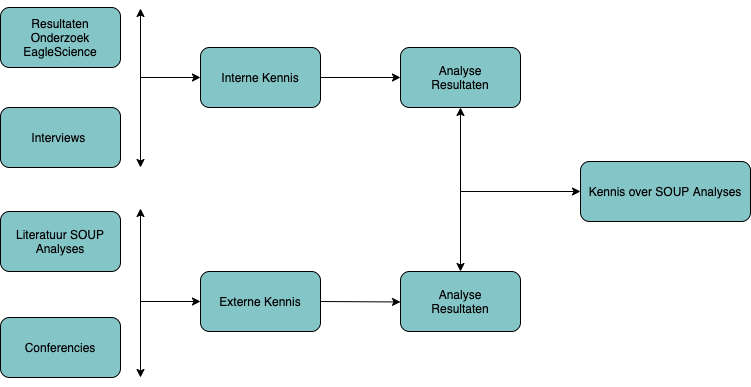
\includegraphics[width=10cm]{gfx/OnderzoeksmodelSOUP}
    \caption{Onderzoeksmodel SOUP analyse module}
    \label{fig:OnderzoeksModelNoodZaakSOUP}
\end{figure}

%
%Dit onderzoek is vooral bedoeld om wegwijs te raken in de wereld het zoeken naar kwetsbaarheden binnen externe bibliotheken.
%Het gaat voornamelijk in op de betekenis van de verschillende begrippen en vervolgens hoe belangrijk het is om deze analyse uit te voeren.
%De uitkomst van dit onderzoek is een basis kennis die als entree voor de komende onderzoeken gebruikt kan worden.
%Het onderzoek heeft niet echt een hoofdvraag waardoor er een duidelijke scope moet worden gedefineerd.
%De volgende zaken moet duidelijk worden in dit onderzoek:
%\begin{itemize}
%  \item "Wat is SOUP?"
%  \item "Waarom kan het gebruik van SOUP gevaarlijk zijn?"
%  \item "Hoe worden deze gevaren/kwetsbaarheden gelogd?"
%  \item "Wat is een CVE en een CVSS?"
%\end{itemize}
%
%
%

\newpage % tijdelijk om te zorgen dat figuur op zelfde pagina als tekst komt
\section{Onderzoek 3: Implementatie van een SOUP-analyse}\label{sec:onderzoek-naar-soup-analyse}
Het \textBF{doel} is om een tooling/bibliotheken te vinden die gebruikt kan worden om soup analyses te doen die binnen de huidige methode van uitrollen van eaglescience past. Daarnaast moet in kaart worden gebracht welke output deze methode genereert zodat het input geeft in de nieuwe oplossing. De \textbf{methode} die gebruikt wordt is deskresearch om te onderzoeken welke tooling er bestaat. Als er een selectie is gemaakt voor een tool dient deze in een kleine testopstelling getest te worden om vervolgens te kijken of we deze kunnen implementeren in de bestaande uitrolmethode. De \textbf{bronnen} die gebruikt zullen worden zijn informatie bronnen van leveranciers van dergelijke tooling. Daarnaast zullen de bevindingen middels een review worden geverifieerd op bruikbaarheid bij de opdrachgever. Het onderzoeksmodel voor dit onderzoek is te vinden in figuur~\ref{fig:OnderzoeksModelSOUPAnalyse}

\begin{figure}[htbp] %Todo: Aanpassen aan het onderzoeksmodel van SOUP analyse
    \myfloatalign
    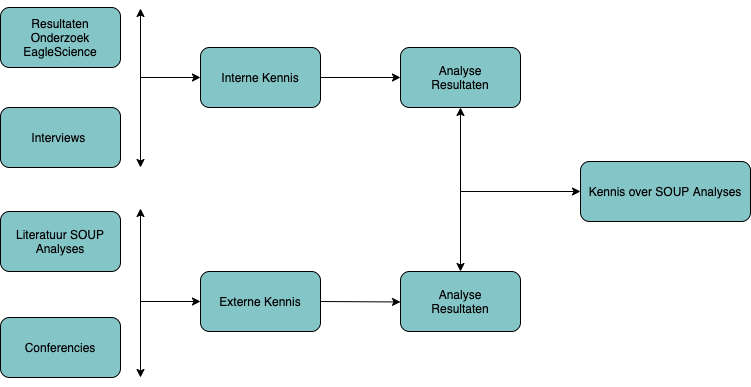
\includegraphics[width=10cm]{gfx/OnderzoeksmodelSOUP}
    \caption{Onderzoeksmodel SOUP analyse module}
    \label{fig:OnderzoeksModelSOUPAnalyse}
\end{figure}
